%%% -*- coding: utf-8 -*-
\newpage

\chapter{Results}
\label{chap:results}

Having performed 20-fold cross validation, we collected all metrics through all the folds. Table \ref{tab:cross-validation-results} presents mean, standard deviation, min and max. The full results for each fold are available on Table \ref{tab:full-folds}, Appendix \ref{chap:appendix}.

\begin{table}[!ht]
\centering
\caption{Weighted F2-Score (in percentage) for each model across 20-Fold Cross Validation).}
\begin{tabular}{l|l|l|l|l}
      & \multicolumn{1}{c|}{MLP} & \multicolumn{1}{c|}{LSTM} & \multicolumn{1}{c|}{SVM} & \multicolumn{1}{c}{KNN} \\ \hline
count & 20,0000                  & 20,0000                   & 20,0000                  & 20,0000                 \\ \hline
mean  & \textbf{99,0743}                  & 98,9899                   & 98,8993                  & 96,4738                 \\ \hline
std   & 0,1349                   & 0,1174                    & 0,1347                   & 0,2915                  \\ \hline
min   & 98,7945                  & 98,7943                   & 98,5445                  & 95,6932                 \\ \hline
25\%  & 99,0073                  & 98,9175                   & 98,8499                  & 96,3585                 \\ \hline
50\%  & 99,0962                  & 98,9848                   & 98,9174                  & 96,4108                 \\ \hline
75\%  & 99,1708                  & 99,0684                   & 98,9756                  & 96,6564                 \\ \hline
max   & 99,2885                  & 99,1915                   & 99,0836                  & 96,9448                
\end{tabular}
\label{tab:cross-validation-results}
\end{table}

Comparing the models in Table \ref{tab:cross-validation-results} the model with the highest Weighed F2-Score is the Multilayer Perceptron model. Although it has the second highest standard deviation, it is still small enough such that the smallest variation still is higher than the second best model, the Long-Short-Term-Memory model.\pva{adicionar teste de diferença significativa}

\begin{figure*}[!ht]
    \centering
    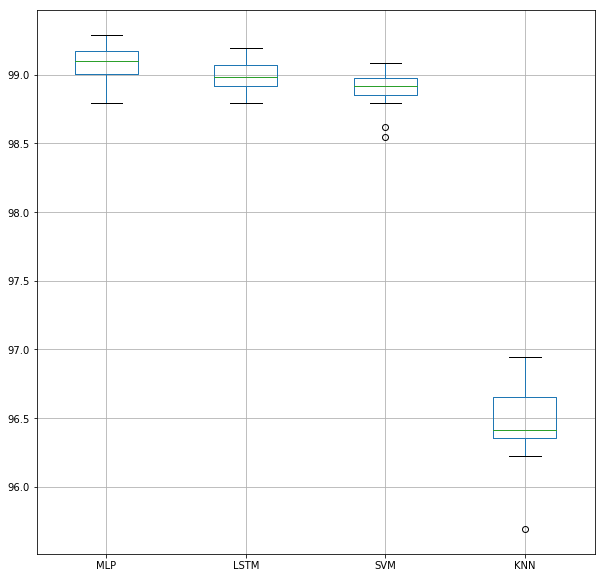
\includegraphics[width=0.5\textwidth]{img/results/boxplot.png}
    \caption{Boxplot of the results of each model throughout the 20-fold cross validation.}
    \label{fig:results-boxplot}
\end{figure*}

\begin{figure*}[!ht]
    \centering
    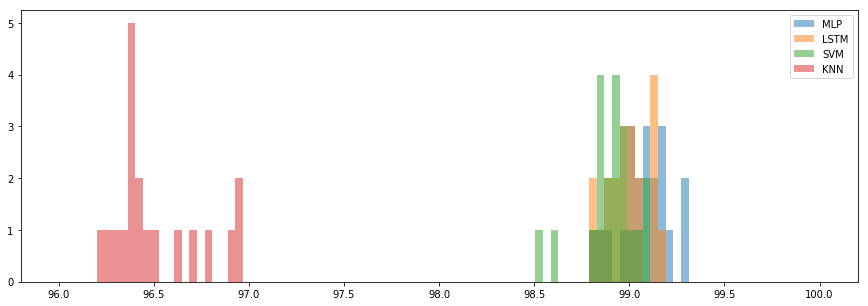
\includegraphics[width=0.9\textwidth]{img/results/histogram.png}
    \caption{Histogram of the results of each model throughout the 20-fold cross validation.}
    \label{fig:results-histogram}
\end{figure*}

Figures \ref{fig:results-boxplot} and \ref{fig:results-histogram}, show the difference in the distribution of results of each model. The simplest model, K-Nearest Neighbors, has the most difference from the models. The three other models, however, are relatively close.

We tested the best performing model, the Multilayer-Perceptron, on the test subset, shown in Table \ref{tab:test-general-results}. 

\begin{table}[!ht]
\centering
\caption{Test subset results, shown in absolute values).}
\begin{tabular}{l|l|l|l|l|l}
             & precision & recall & f1-score & f2-score & support                         \\ \hline
Safe         & 0,9895    & 0,9906 & 0,9900   & 0,9897   & 5973,0000                       \\ \hline
Sensitive    & 0,9906    & 0,9895 & 0,9900   & 0,9904   & 5973,0000                       \\ \hline
weighted avg & 0,9900    & 0,9900 & 0,9900   & 0,9900   & \multicolumn{1}{l}{11946,0000}
\end{tabular}
\label{tab:test-general-results}
\end{table}

As shown in Table \ref{tab:test-general-results} and in Figure \ref{fig:cf-test}, the MLP model has performed within the range of the mean of the cross validation. It can also be noted that, the most frequent errors were \textit{false positives}, when the model predicted a video as Sensitive when it was in fact, Safe. 

\begin{figure*}[!ht]
    \centering
    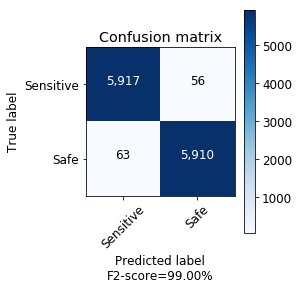
\includegraphics[width=0.49\textwidth]{img/results/MLP-TEST.png}
    \caption{Confusion matrix of the predictions of the best model in the test subset.}
    \label{fig:cf-test}
\end{figure*}

We also tested our best model in each sub task, pornography and gore binary classification. For the pornography, shown in Table \ref{tab:test-porn-results}, and Figure \ref{fig:cf-test-porn}, the most frequent error were the \textit{false negatives}, in which the model predicted that the most samples were predicted as Safe, but were actually Sensitive. 

\begin{table}[!ht]
\centering
\caption{Results testing pornography only, shown in absolute values).}
\begin{tabular}{l|l|l|l|l|l}
             & precision & recall & f1-score & f2-score & support    \\ \hline
Safe         & 0,9947    & 0,9902 & 0,9925   & 0,9939   & 5737,0000  \\ \hline
Sensitive    & 0,9903    & 0,9948 & 0,9925   & 0,9911   & 5737,0000  \\ \hline
weighted avg & 0,9925    & 0,9925 & 0,9925   & 0,9925   & 11474,0000
\end{tabular}
\label{tab:test-porn-results}
\end{table}

For the gore, shown in Table \ref{tab:test-gore-results}, and Figure \ref{fig:cf-test-gore}, the most frequent error were the \textit{false positive}, in which the model predicted that the most samples were predicted as Sensitive, but were actually Safe.  

\begin{table}[!ht]
\centering
\caption{Results testing gore videos only, shown in absolute values).}
\begin{tabular}{l|l|l|l|l|l}
             & precision & recall & f1-score & f2-score & support  \\ \hline
Safe         & 0,8764    & 0,9915 & 0,9304   & 0,8834   & 236,0000 \\ \hline
Sensitive    & 0,9902    & 0,8602 & 0,9206   & 0,9661   & 236,0000 \\ \hline
weighted avg & 0,9333    & 0,9258 & 0,9255   & 0,9248   & 472,0000
\end{tabular}
\label{tab:test-gore-results}
\end{table}

\begin{figure*}[!ht]
    \centering
    \begin{subfigure}[b]{0.49\textwidth}
        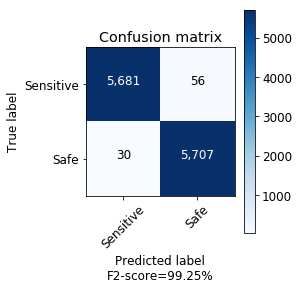
\includegraphics[width=0.93\textwidth]{img/results/MLP-TEST-PORN.png}
        \caption{Confusion matrix of the model on the pornography videos of the test subset.}
        \label{fig:cf-test-porn}
    \end{subfigure}
    \begin{subfigure}[b]{0.49\textwidth}
        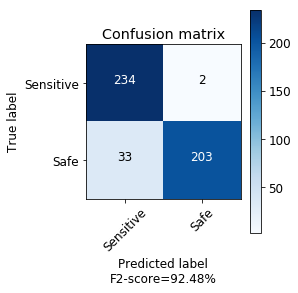
\includegraphics[width=0.90\textwidth]{img/results/MLP-TEST-GORE.png}
        \caption{Confusion matrix of the model on the gore videos of the test subset.}
        \label{fig:cf-test-gore}
    \end{subfigure}
    \caption{Confusion matrices of the best performing model on the pornography and gore subsets.}
\end{figure*}

To evaluate if our model and our dataset on the pornography detection (binary classification) task, we also tested our best performing baseline model on a well known dataset for pornography detection: The 2k-pornography dataset. The results are shown in \ref{tab:test-2k-results} and in Figure \ref{fig:cf-test-2k}. The most common errors were false negatives, in which the model predicts the instance as a Safe, but the true label were Sensitive.

\begin{table}[!ht]
\centering
\caption{Test on the NPDI 2k-pornography dataset results, shown in absolute values).}
\begin{tabular}{l|l|l|l|l|l}
             & precision & recall & f1-score & f2-score & support    \\ \hline
Safe         & 0,9665    & 0,8080 & 0,8802   & 0,9411   & 1.000,0000 \\ \hline
Sensitive    & 0,8351    & 0,9720 & 0,8983   & 0,8354   & 1.000,0000 \\ \hline
weighted avg & 0,9008    & 0,8900 & 0,8893   & 0,8883   & 2.000,0000
\end{tabular}
\label{tab:test-2k-results}
\end{table}

\begin{figure*}[!ht]
    \centering
    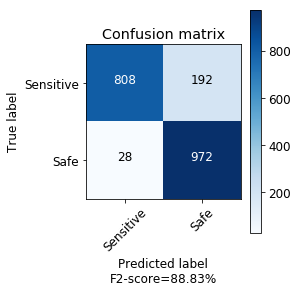
\includegraphics[width=0.49\textwidth]{img/results/MLP-2K-TEST.png}
    \caption{Confusion matrix of the predictions of the best model in the NPDI 2k-pornography dataset.}
    \label{fig:cf-test-2k}
\end{figure*}


\section{Discussion}\label{sec:discussion}
% Falar dos resultados de teste e de cada task
% Para tarefas de porn, o mais comum foram falsos negativos, como esperado
% Para tarefas  de gore, o mais comum foram falsos positivos, que previram como sensivel mas eram safe, que é o idela, mas pq esses videos sao bem parecidos com safe
% Falar dos erros do pornography2k, que usou f2 score, de quanto foi o modelo deles, e dos erros mais comuns (Falsos negativos) 
% Falar pq isso aconteceu, qual a diferença entre os dois datasets e os modelos
% por eles usarem late fusion talvez tenha ajudado, especialmente pq o nosso modelo usa só as features de imagem
\section{Analysis cases}\label{sec:experiments-discussion}

In order to further investigate the impact of each multi-modal feature in our best performing model, the Multilayer Perceptron, we tested it on our test subset and on the NPDI 2k-pornography dataset, but only using one modal feature at a time. For example, in Figure \ref{fig:cf-test-image}, we tested the MLP model using only visual (frames) features, specifically, were changed all audio features for zero to simulate a video with no audio features.

\begin{figure*}[!ht]
    \centering
    \begin{subfigure}[b]{0.49\textwidth}
        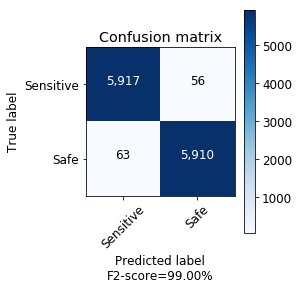
\includegraphics[width=0.94\textwidth]{img/results/MLP-TEST-IMAGE-ONLY.png}
        \caption{Confusion matrix of the model on the test subset using only image features.}
        \label{fig:cf-test-image}
    \end{subfigure}
    \begin{subfigure}[b]{0.49\textwidth}
        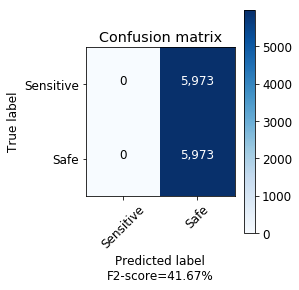
\includegraphics[width=0.94\textwidth]{img/results/MLP-TEST-AUDIO-ONLY.png}
        \caption{Confusion matrix of the model on the test subset using only audio features.}
        \label{fig:cf-test-audio}
    \end{subfigure}
    \caption{Confusion matrices of the model on the test subset using only one multi-modal feature at a time.}
\end{figure*}

As observed in Figures \ref{fig:cf-test-image} and \ref{fig:cf-test-audio}, our model had the same performance with only visual features, but mis-classified all Sensitive videos. This means that the MLP model ignored all audio features for all videos. It is relying only in visual features, even though there are examples of videos in the dataset, in which the main feature of a sensitive video is audio. % ASMr VIDEOS

\begin{figure*}[!ht]
    \centering
    \begin{subfigure}[b]{0.49\textwidth}
        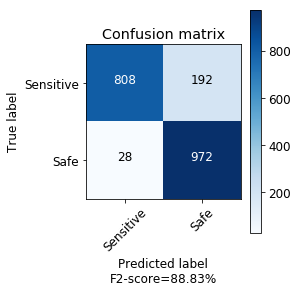
\includegraphics[width=0.94\textwidth]{img/results/MLP-2K-TEST-IMAGE-ONLY.png}
        \caption{Confusion matrix of the model on the NPDI 2k-pornography dataset using only image features.}
        \label{fig:cf-test-2k-image}
    \end{subfigure}
    \begin{subfigure}[b]{0.49\textwidth}
        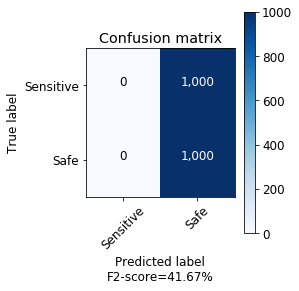
\includegraphics[width=0.94\textwidth]{img/results/MLP-2K-TEST-AUDIO-ONLY.png}
        \caption{Confusion matrix of the model on the NPDI 2k-pornography dataset using only audio features.}
        \label{fig:cf-test-2k-audio}
    \end{subfigure}
    \caption{Confusion matrices of the model on the NPDI 2k-pornography dataset using only one multi-modal feature at a time.}
\end{figure*}

We confirmed this pattern with the test with the NDPI 2k-pornography dataset, as shown in Figures \ref{fig:cf-test-2k-image} and \ref{fig:cf-test-2k-audio}.%, our model relied only in visual features.

% Discutir vantagens e desvantagens do eraly fusion por causa de forçar o modelo a aprender uma mdeia de cada e depois combinar
% Possibilidades pra so ter aprendido imagens:
%Diferença no tamanho das deatures de audio e frames
%Diferença pra early e late fusion
%Só a mlp aprendeu isso
%Features ruins de audio
% Receptive field pra áudio pequeno
% Audio n faz diferença ***: perguntar pra paulo oq ele quis dizer
